\section{\texorpdfstring{\logic Neural-symbolic Integration for Attack Detection}{Neural-symbolic Integration for Attack Detection}}

% Legend item style for metro map overlay
\tikzset{legenditem/.style={
    %fill=white,
    %draw=gray!30,
    %rounded corners=2pt,
    inner ysep=1pt,
    inner xsep=3pt,
    %outer sep=0pt,
    minimum width=12.5em,
    text width=12.5em,
    font=\scriptsize,
    %align=left,
    anchor=north west
}}
\tikzset{largeitem/.style={
    legenditem,
    minimum width=20em,
    text width=20em,
}}
\tikzset{citeitem/.style={
    inner sep=3pt,
    text width=0.75\textwidth,
    font=\scriptsize,
    yshift=.2ex,
}}

\begin{frame}%{Contributions overview -- PhD}

  \alt<2->{\frametitle{Contributions overview -- Postdoc}}{\frametitle{Contributions overview -- PhD}}

  \begin{tikzpicture}[remember picture, overlay, shift={(current page.south west)}, x=\paperwidth, y=\paperheight]%
    \node[anchor=south, yshift=-5pt] at (current page.south) {
      \foreach \i in {4,5,5,6,7,8} {%
        \includegraphics<+>[height=.95\textheight]{figures/metro/\i.pdf}%
      }%
      \includegraphics<+>[height=.95\textheight]{figures/metro/8-transparent.pdf}%
    };

    \alt<1-5>{
      \node[legenditem] (legend-0-0) at (0.02,0.3) {\hspace{1.4em}\textbf{CONTRIBUTIONS}};
      \node[legenditem] (legend-0-1) at (legend-0-0.south west) {\slr \texttt{Survey (SLR)}~\autocite{lavaur_tnsm_2022,lavaur_cesar_2022}};
      \node[legenditem] (legend-0-2) at (legend-0-1.south west) {\eiffel \texttt{Assessment \& eiffel}~\autocite{lavaur_icdcs_demo_2024,lavaur_ares_bass_2024,lavaur_cose_2025}};
      \node[legenditem] (legend-0-3) at (legend-0-2.south west) {\radar \texttt{RADAR}~\autocite{lavaur_radar_2024,lavaur_algotel_2025}};
      \node[legenditem] (legend-0-4) at (legend-0-3.south west) {\feditn \texttt{FedITN}~\autocite{lavaur_anubis_2025}};
    }{
      \node[legenditem, opacity=0.3] (legend-0-0) at (0.02,0.3) {\hspace{1.4em}\textbf{CONTRIBUTIONS}};
      \node[legenditem,opacity=0.3] (legend-0-1) at (legend-0-0.south west) {\slr \texttt{Survey (SLR)}~\autocite{lavaur_tnsm_2022,lavaur_cesar_2022}};
      \node[legenditem,opacity=0.3] (legend-0-2) at (legend-0-1.south west) {\eiffel \texttt{Assessment \& eiffel}~\autocite{lavaur_icdcs_demo_2024,lavaur_ares_bass_2024,lavaur_cose_2025}};
      \node[legenditem,opacity=0.3] (legend-0-3) at (legend-0-2.south west) {\radar \texttt{RADAR}~\autocite{lavaur_radar_2024,lavaur_algotel_2025}};
      \node[legenditem,opacity=0.3] (legend-0-4) at (legend-0-3.south west) {\feditn \texttt{FedITN}~\autocite{lavaur_anubis_2025}};
    }

    \only<2-5>{
      \node[legenditem,yshift=-.3ex] (legend-0-5) at (legend-0-4.south west) {\hspace{1.4em}\textbf{ONGOING WORK}};
      \node[largeitem] (legend-0-6) at (legend-0-5.south west) {\flb \texttt{Gossip learning for WSNs\textsuperscript{$\ddagger$}}};
    }
    \only<6>{
      \node[legenditem,yshift=-.3ex,opacity=0.3] (legend-0-5) at (legend-0-4.south west) {\hspace{1.4em}\textbf{ONGOING WORK}};
      \node[largeitem,opacity=0.3] (legend-0-6) at (legend-0-5.south west) {\flb \texttt{Gossip learning for WSNs\textsuperscript{$\ddagger$}}};
    }
    \only<2>{
      \node[citeitem, anchor=south east] at (current page.south east) {\textsuperscript{$\ddagger$}~Collab. with \textexample{H. Rivano} (INSA Lyon; Citi/Agora). One submission.};
    }
    \only<3>{
      \node[fill=white, opacity=0.5, minimum width=\paperwidth, minimum height=\paperheight] at (current page.center) {};
      \node[anchor=center, draw=gray, rounded corners=3pt, inner sep = 10pt, fill=white] at (current page.center) {
        \begin{minipage}{.8\paperwidth}
          \textbf{COCTEL: Causality-Oriented Cybersecurity TELemetry}~\logic~\waterllmarks
          \begin{itemize}
            \item \alert{\bfseries Goal:} how to extract and represent relationships between distributed events, allowing forward and backward reasoning about them.
            \item Academic project, FNR funding (Luxembourgish national research fund), PI: Jérôme François (SnT).
          \end{itemize}
      \end{minipage}};
      \node[anchor=south east, xshift=-1em, yshift=1em] at (current page.south east) {%
        \raisebox{-0.5\height}{
\includegraphics[height=1.2cm]{assets/logos/SnT_UL_colour.pdf}}%
        \hspace{-.5em}\raisebox{-0.5\height}{
\includegraphics[height=1cm]{assets/logos/FNR_LOGO_BIG.pdf}}%
      };
    }

    \only<4-6>{
      \node[legenditem,anchor=north west] (legend-1-1) at (legend-0-1.north east) {\waterllmarks \texttt{WaterLLMarks}~\autocite{lavaur_waterllmarks_2025}};
    }
    \only<4>{
      \node[citeitem, anchor=south east] at (current page.south east) {\smallfullcite{lavaur_waterllmarks_2025}. Demo track ICDCS.};
    }
    \only<7->{
      \node[legenditem,opacity=0.3,anchor=north west] (legend-1-1) at (legend-0-1.north east) {\waterllmarks \texttt{WaterLLMarks}~\autocite{lavaur_waterllmarks_2025}};
    }

    \only<5-6>{
      \node[largeitem] (legend-1-2) at (legend-1-1.south west) {\rag \texttt{Semantic access control for RAG}~\autocite{thuillier_aiml_2026}};
    }
    \only<5>{
      \node[citeitem, anchor=south east] at (current page.south east) {\smallfullcite{thuillier_aiml_2026}};
    }
    \only<7->{
      \node[largeitem,opacity=0.3] (legend-1-2) at (legend-1-1.south west) {\rag \texttt{Semantic access control for RAG}~\autocite{thuillier_aiml_2026}};
    }

    \only<6->{
      \node[largeitem] (legend-1-3) at (legend-1-2.south west) {\logic \texttt{Logic and neural-symbolic integration}~\autocite{anser_fmano_2026}};
    }
    \only<6>{
      \node[citeitem, anchor=south east] at (current page.south east) {\smallfullcite{anser_fmano_2026}};
    }

  \end{tikzpicture}%
\end{frame}

%  1. Définitions/Context : raisonnement symbolique, intégration neuro symbolique
% - comp type 1/2
% - interpretability and determinism when needed
\begin{frame}[t]{Definitions}
  \begin{block}{Symbolic reasoning}
    Represents knowledge as explicit symbols (\alert{facts}) and provides \alert{rules} to derive new knowledge or make decisions.
    \pause
    Example of rule in First-Order Logic (FOL):
    \begin{equation*}
      \forall p,f: \text{IsShellProcess}(p) \land \text{Accesses}(p,f) \land \text{IsSensitiveFile}(f) \rightarrow \text{IsSuspicious}(p).
    \end{equation*}
  \end{block}

  \pause
  \begin{block}{Neural-symbolic integration}
    Combines symbolic reasoning (interpretability, explicit knowledge representation) with neural networks (learning from data, handling uncertainty). \Eg, DeepProbLog~\footcite{manhaeve_DeepProbLogNeuralProbabilistic_2018}, Scallop~\footcite{li_ScallopLanguageNeurosymbolic_2023}.
  \end{block}
\end{frame}

% 2. It all starts from a dataset...
% - casino limit
% - our goal, extract relationships between attacks
\begin{frame}{It all starts from a dataset\dots}
  \begin{columns}
    \column{0.5\textwidth}

    \textbf{The CasinoLimit dataset}~\autocite{kilian_CasinoLimitOffensiveDataset_2025}
    \begin{itemize}
      \item Controlled CTF exercise played by 114 participants, each on an isolated but identical instance.
      \item A defined 8-step scenario labeled with MITRE ATT\&CK techniques.
        \pause
      \item \alert{Our goal:} extract the scenario from the data, using classification and domain knowledge.
    \end{itemize}

    \column{0.5\textwidth}
    \vspace{-.5em}
    \centering
    \only<3>{\vspace{-2em}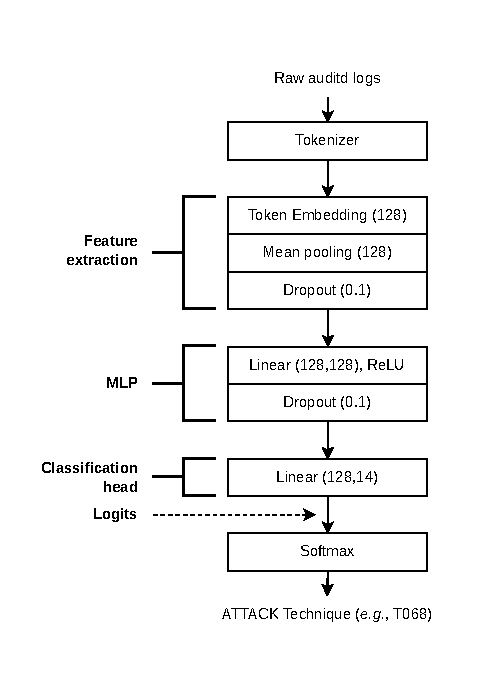
\includegraphics[width=.75\textwidth]{figures/postdoc/nesy/mlp.drawio.pdf}}%
    \includegraphics<4>[width=1.05\textwidth,center]{figures/postdoc/nesy/confmat}%
    \vfill
  \end{columns}
  \footcite*{kilian_CasinoLimitOffensiveDataset_2025}
\end{frame}

% 4. Adding contexte (arch neuro sym with animations)
% - usually in ml we do window (mention lstm/transformer)
% - logit rerank at inference

\begin{frame}{Adding Context with Symbolic Rules}
  \begin{columns}
    \column{0.5\textwidth}
    \begin{itemize}[<+->]
      \item Use a rolling window of events to capture context.
      \item Typically implemented with LSTMs or Transformers.
      \item Automatically derive rules instead.
      \item Rerank model outputs at inference time.
    \end{itemize}

    \column{0.5\textwidth}
    \centering
    \includegraphics<1>[height=.95\textheight]{figures/postdoc/nesy/arch-1.drawio.pdf}%
    \includegraphics<2>[height=.95\textheight]{figures/postdoc/nesy/arch-lstm.drawio.pdf}%
    \includegraphics<3>[height=.95\textheight]{figures/postdoc/nesy/arch-2.drawio.pdf}%
    \includegraphics<4>[height=.95\textheight]{figures/postdoc/nesy/arch-4.drawio.pdf}%
  \end{columns}
\end{frame}

% 5. Integrating at train time (old figure or new if time)
\begin{frame}{Different Types of Integration}
  \centering
  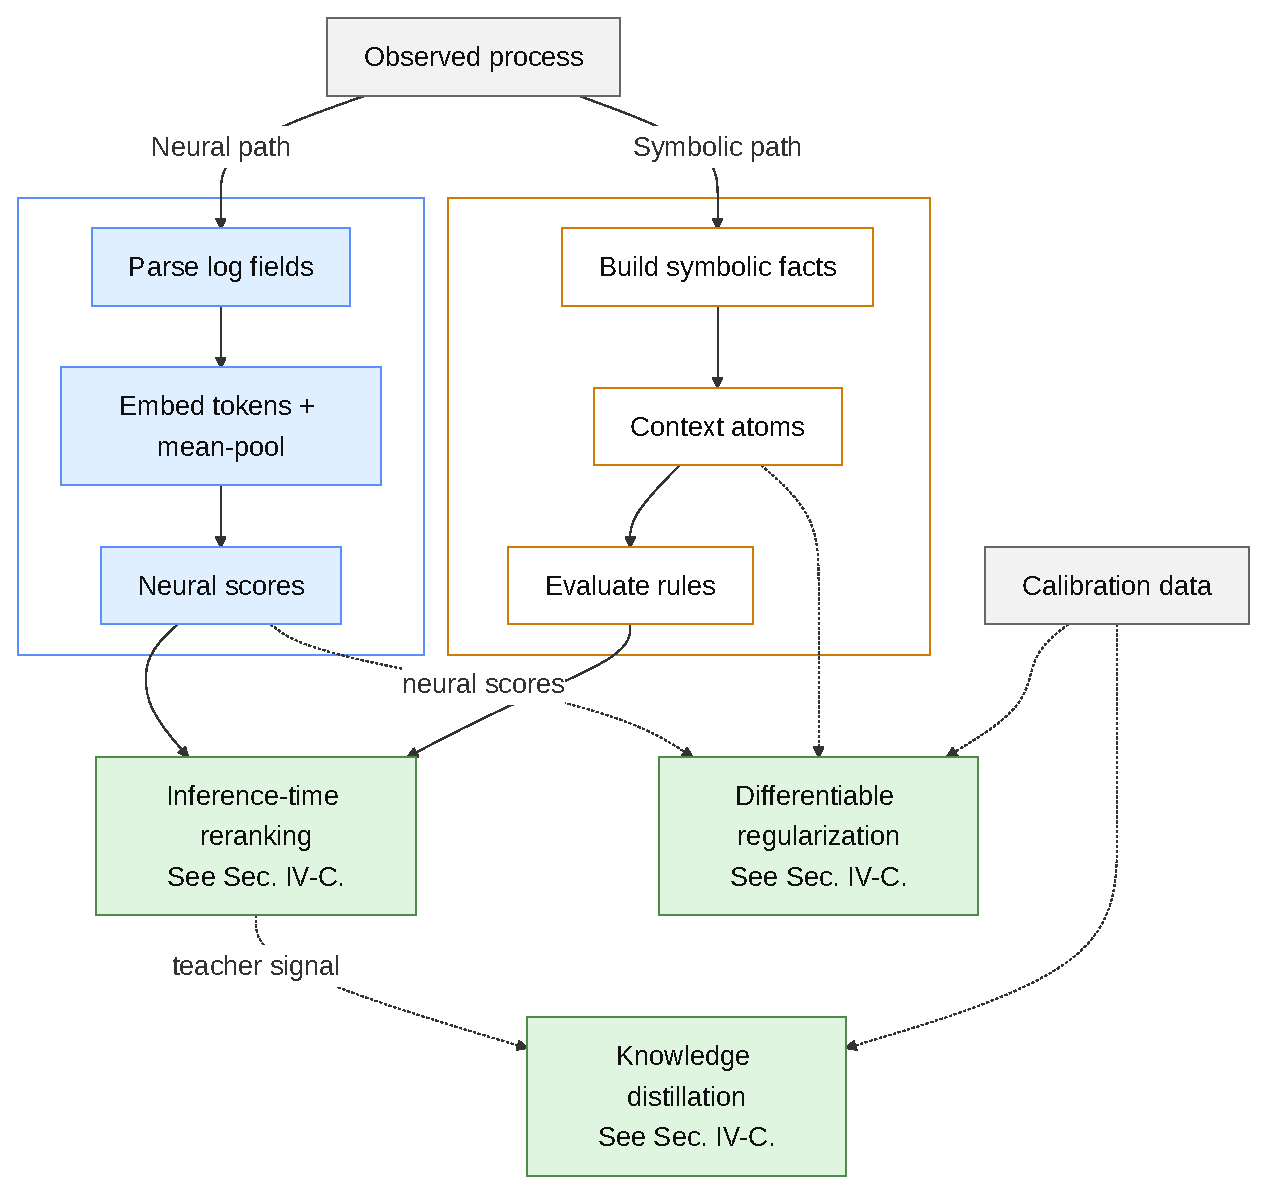
\includegraphics[width=.6\textwidth]{figures/postdoc/nesy/methodology_overview_cropped.pdf}%
\end{frame}

% 6. Results
{\setbeamercovered{transparent}
  \begin{frame}{Results}
    \centering
    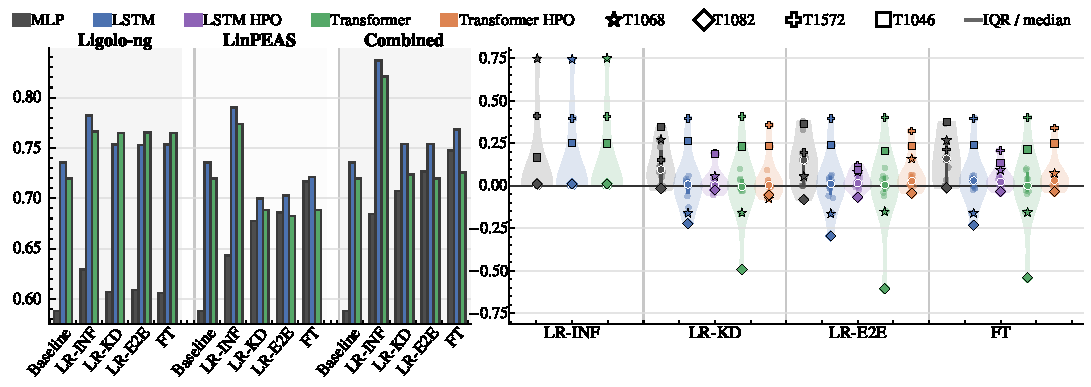
\includegraphics[width=0.9\textwidth]{figures/postdoc/nesy/results.pdf}
    \vspace{-0.8em}
    \begin{description}
        {\only<2>{\transparent{0.3}}%
      \item[Left:] Macro-F1 across backbones and integration methods: train-time outperforms inference-time, and can match LSTM/Transformer performance with a simple MLP backbone.}
        {\only<1>{\transparent{0.3}}%
      \item[Right:] Per-technique $\Delta$F1 versus the corresponding baseline: inference-time correction provide very consistent improvements across techniques.}
    \end{description}
  \end{frame}
}
% 7. Interests for Collab
% - inf time adaptation
% - auditability by interpretability
% - train smaller models and join With logic
\begin{frame}{Takeways}
  \begin{block}{Convincing proof of concept}
    Can effectively leverage \alert{domain knowledge} to improve performance, particularly with simple backbones.
  \end{block}

  \pause
  \begin{block}{Improved auditability}
    Symbolic rules provide \alert{interpretability} and can be used to audit model decisions.
  \end{block}

  \pause
  \begin{block}{Scaling problem}
    Automatic rule derivation is necessary to scale to more behaviors and scenarios.\pause{} \alert{Derive from provenance graphs?}
  \end{block}
\end{frame}